\section{Introduction}
\begin{quote}
    \citep{pml1Book} -- Chapter 1.
\end{quote}

\subsection{Supervise Learning}
\textbf{Probabilistic perspective} ML: treat all unknown quantities as r.v.s.
endowed probability distribution describing a weighted set of the possible values.

\begin{note}
    Why is the probabilistic perspective adopted?
    \begin{enumerate}
        \item decision making under uncertainty and
        \item general language by other fields of science and engineering.
    \end{enumerate}
\end{note}


\textbf{Empirical risk} is the function of parameters $\bm{\theta}$, 
where the term \textit{empirical} implies using sample average to substitute population-level expectation 
(real data distribution is usually unknown), 
and the loss function $\ell(\cdot)$ can be specified according to real-world condition.
The model fitting is to find a \underline{minimizer} $\hat{\bm{\theta}}$ of $\mathcal{L}(\bm{\theta})$.
\begin{gather}
    \mathcal{L}(\bm{\theta})=\frac{1}{N}\sum_{n=1}^N
    {\ell(y_n,f(\bm{x}_n;\bm{\theta}))}
\end{gather}

\textbf{Conditional probability distribution} is adopted to capture the uncertainty.
\begin{gather}
    p(y|\bm{x};\bm{\theta})
    =f_y(\bm{x};\bm{\theta}):\mathcal{X}\to\mathcal{Y}
\end{gather}

\textbf{Deep neural networks} (vs linear\&polynomial regression) do 
nonlinear feature extraction automatically with stacked multiple hidden layers $\phi(\cdot;\bm{V})$
with $\bm{V}=[\bm{\theta}_1,\cdots,\bm{\theta}_{L-1}]$ 
and output the prediction with the final layer with $\bm{w}=\bm{\theta}_L$.
\begin{gather}
    f(\bm{x};\bm{w},\bm{V})=\bm{w}^T\phi(\bm{x};\bm{V})
\end{gather}

\begin{quote}\textit{
    Supervised learning is essentially just ``glorified curve fitting''.
}\end{quote}

\subsection{Unsupervised learning}

\textit{Unconditional} vs \textit{conditional}\unsure{
$\bm{y}$ follows mixed model with additional uncertainty of unknown co-variates
introduced by transformation from $\bm{x}$
}
models of \textit{unsupervised} vs \textit{supervised} learning.
\begin{gather}
    p(\bm{x})~\text{vs}~p(\bm{y}|\bm{x})
\end{gather}

% \begin{note}
    Strategies to find such model $p(\bm{x})$ generating data:
    \begin{enumerate}
        \item clustering by defining the similarity (distance in same space) among data points; 
        \item modeling the low-dimensional representation (Equation (\ref{eq:latent})) 
        of unobserved latent factors;
        \item self-supervised learning: 
        build proxy supervised tasks from unlabeled data, and 
        learn useful representation from the data themselves.
    \end{enumerate}
% \end{note}

\begin{example}
    \textbf{Modeling low-dimensional latent representation}\\
    \begin{gather}
        p(\bm{x}_n|\bm{z}_n;\bm{\theta})
        =N(\bm{x}_n|f(\bm{z}_n;\bm{\theta}),\bm{\Sigma})
        ~~~\bm{z}_n\in\mathbb{R}^K,~K\ll{D}
        \label{eq:latent}
    \end{gather}
    \begin{itemize}
        \item \textbf{Factor analysis}: 
        $f(\bm{z}_n;\bm{\theta})=\bm{W}\bm{z}_n+\bm{\mu}$
        \item \textbf{PCA}:
        $f(\bm{z}_n;\bm{\theta})=\bm{W}\bm{z}_n+\bm{\mu}$ and 
        $\bm{\Sigma}=\sigma^2\bm{I}$
        \item \textbf{Variational autoencoder}:
        $f(\cdot)$ neural network (nonlinear) and
        $\bm{\Sigma}=\sigma^2\bm{I}$
    \end{itemize}
\end{example}

Principles of evaluating unsupervised learning
\begin{enumerate}
    \item \textit{data compression as lossless as possible}:
    treat it as density estimation\unsure{
    recall the knowledge learned from \textit{Statistical Inference}}
    and see if a model captures the typical and useful patterns in the data;
    \item \textit{sample efficiency} of the learned representation: improvement in downstream application, 
    say, supervised learning tasks (easy to evaluate);
    \item \textit{interpretability}: discover the true underlying structure behind some dataset.
\end{enumerate}

\subsection{Reinforcement Learning}
\begin{figure}[htpb]
    \centering
    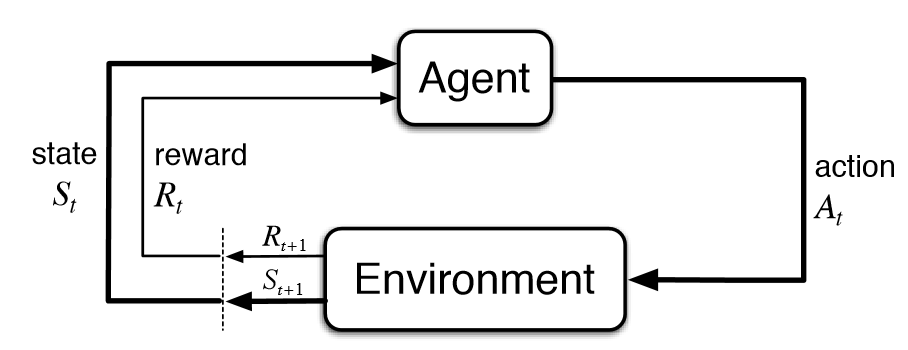
\includegraphics[width=0.7\textwidth]{figs/rl.png}
    \caption{Reinforcement Learning\protect\footnotemark[1]}
    \label{fig:rldiag}
\end{figure}
\footnotetext[1]{
\hyperlink{https://towardsdatascience.com/reinforcement-learning-101-e24b50e1d292}
{https://towardsdatascience.com/reinforcement-learning-101-e24b50e1d292}}

% \begin{quote}
%     Some key terms that describe the basic elements of an RL problem are\footnotemark[1]:
%     \begin{itemize}
%         \item Environment: Physical world in which the agent operates
%         \item State: Current situation of the agent
%         \item Reward: Feedback from the environment
%         \item Policy: Method to map agent’s state to actions
%         \item Value: Future reward that an agent would receive by taking an action in a particular state
%     \end{itemize}
% \end{quote}

Compared with supervised learning, the reward in RL may only be given occasionally and summarily
(e.g. if the agent eventually reaches a desired state after a path of actions)

\subsection{Data}

Common datasets (Benchmark):
\begin{itemize}
    \item small image datasets: MNIST [1,28,28] (extend to EMNIST, fashion-MNIST), CIFAR-10 [3,32,32];
    \item large image datasets: ImageNet [3,256,256];
    \item text datasets for text classification: IMDB movie review dataset;
    \item text datasets for machine translation: documents from multilingual organizations 
    (e.g. Canadian parliament and EU), WMT dataset;
    \item seq2seq tasks (e.g. document summarication and question answering): ?.
\end{itemize}

\textbf{TF-IDF}: term frequency-inverse document frequency.\unsure{
weighted BoW that reduce the importance of uninformative terms
}
TF$_{ij}$ is the frequency of term $i$ in document $j$, and 
IDF$_i\triangleq{\frac{N}{1+\text{DF}_i}}$, 
where $DF_i$ is the number of documents with term $i$.
\begin{gather}
    \text{TF-IDF}_{ij}=\log{\text{TF}_{ij}+1}\times\text{IDF}_i
\end{gather}

\textbf{Word embeddings}: 
\unsure{
Usually self-supervised models were adopted to build a pre-trained word embeddings 
based on large-scale contexts.
}\unsure{
The embeddings with similar meanings be often close in some metric space.}
map sparse and vocabulary-length (high-dimensional) vectors to 
dense and low-dimensional ones (embeddings).

Strategies to deal with OOV:
\begin{enumerate}
    \item replace all novel words with $\mathtt{UNK}$;
    \item byte-pair encoding: finer-grained subword structure embedding;
\end{enumerate}

Let $\bm{M}\in\mathbb{I}^{N\times{D}}$ indicates the missing status of feature $\bm{X}$:
$M_{nd}=1$ if $X_{nd}$ is missing and let $\bm{X}_v~(\bm{M}_v=\bm{0})$ and 
$\bm{X}_h~(\bm{M}_h=\bm{1})$ 
are visible and missing parts of features, respectively. 
The outcome labels $\mathbf{Y}$ are full observed.\unsure{
Missing data handling is a complex topic,
also important in \textit{clinical trial designing}, 
and will be discussed later and further.
}
\begin{itemize}
    \item \textbf{missing completely at random} (MCAR): 
    $p(\bm{M}|\bm{X}_v,\bm{X}_h,\bm{Y})=p(\bm{M})$,
    the missingness does not depend on the hidden/observed features;
    \item \textbf{missing at random} (MAR):
    $p(\bm{M}|\bm{X}_v,\bm{X}_h,\bm{Y})
    =p(\bm{M}|\bm{X}_v,\bm{Y})$,
    the missingness does not depend on the hidden features but may depend on the visible features;
    \item \textbf{not missing at random} (NMAR): otherwise
\end{itemize}

\begin{note}
    In the MCAR/MAR case, the missingness mechanism can be ignored since missingness is
    independent with the unobserved features. 
    And \textbf{this book always makes the MAR assumption}.
\end{note}

\section{Foundations}
\begin{quote}
    \citep{pml1Book} -- Chapter 2-8.
\end{quote}

\subsection{Probability: Univariable and Multivariable Models}

Types of uncertainty:
\begin{enumerate}
    \item \textbf{model uncertainty}: or epistemic uncertainty,
    caused by our ignorance of the underlying hidden causes or mechanism generating the data;
    \item \textbf{data uncertainty}: or aleatoric uncertainty,
    caused by intrinsic variability (the true model generating data randomly).
\end{enumerate}

Paradigm of binary classification with the assumption of probability output:
\begin{gather}
    p(y|\bm{x},\bm{\theta})
    =\text{Bernoulli}(y|\sigma(f(\bm{x};\bm{\theta})))
\end{gather}
where basic property of neuron, activation function $\sigma(a)$, in a network's output layer is compressing the value of unconstrained function to $[0,1]$, 
one example with good characteristics (refer to \citep{pml1Book} Table 2.3) 
of which is the sigmoid function $\frac{1}{1+e^{-a}}$, 
and the variety of $f$'s contributes to the contemporary blossom of deep learning architectures, 
the easiest one of which is linear model $\bm{w}^T\bm{x}+b$. (Logistic regression: Binomial+Sigmoid \& Multinomial+Softmax
\unsure{log-sum-exp trick for computer friendly to avoid floating-point overflow})

Paradigm of regression:
\begin{gather}
    p(y|\bm{x};\bm{\theta})
    =\mathcal{N}(y|
    f_\mu(\bm{x};\bm{\theta}),
    f_\sigma^2(\bm{x};\bm{\theta})
    )
\end{gather}
where $f_\mu\in\mathbb{R}$ predicts the mean 
and $f_\sigma^2\in\mathbb{R}^+$ predicts the variance.
Recall the two types of uncertainty,
the \textbf{uncertainty of data} ($y$) is presented by $f_\sigma(\bm{x};\bm{\hat{\theta}})$ and 
the \textbf{uncertainty of model} ($\bm{\theta}$) is presented by 
$\mathrm{Var}f_\mu(\bm{x};\bm{\theta})$.

Gaussian (or Normal) distribution has good characteristics
\begin{enumerate}
    \item with two parameters $\mu,\sigma^2$, easy to interpret;
    \item by central limit theorem (modeling the noise from multiple sources);
    \item with the least number of assumptions;
    \item with simple form, easy to implement but highly effective.
\end{enumerate}

\textbf{Heavy-tail} distributions, say, 
Student, Cauchy, and Laplace (double sided Exp.) distributions, 
is robust to outliers.\unsure{
Grafting of Normal main body and Cauchy tails are also used to deal with outliers like RCTD.
} 
It is common to set $\nu=4$, if greater, then Student dist. approaches to $\mathcal{N}$.

\textbf{Monte Carlo approximation}. 
Consider an arbitrary transformation $\bm{Y}=g(\bm{X})$,
it is often difficult to compute the induced distribution $f_{\bm{Y}}(\bm{y})$ analytically,
but it can be approached by drawing a large amount of samples 
from the original distribution $f_{\bm{X}}(\bm{x})$:
\begin{gather}
    f_{\hat{\bm{Y}}}(\bm{y})
    \triangleq
    \frac{1}{N}\sum_{s=1}^N\delta(\bm{y}-g(\bm{x}_s))
\end{gather}



% \begin{framed}{\Large

% TODO list in the following week
% \begin{itemize}
%     \item Finish reading the remaining chapters in the Foundation part
%     \item Finish reading \citep{shao2003mathematical} and 
%     do the exercises (for STAT5005)
%     \item Finish organizing the hand writing notes of STAT5010.
% \end{itemize}

% }\end{framed}
\textbf{Simpson's paradox} says that a statistical trend or relationship 
that appears in several difficult groups of data can disappear or reverse sign 
when these groups are combined.

\textbf{Convariance} of multiple r.v.. $\bm{X}=(X_1,\cdots,X_D)$ is defined as\unsure{
Useful in Multivariate Analysis and Linear Model
} 
\begin{align}
    \bm{\Sigma}\triangleq\mathrm{Cov}\bm{X}
    =& \mathbb{E}\left[
    (\bm{X}-\mathbb{E}\bm{X})
    (\bm{X}-\mathbb{E}\bm{X})^T
    \right]\\
    =& \mathbb{E}[\bm{XX}^T]-[\mathbb{E}\bm{X}][\mathbb{E}\bm{X}]^T
\end{align}
\begin{enumerate}
    \item $\mathbb{E}[\bm{XX}^T]=\bm{\Sigma}+\bm{\mu}\bm{\mu}^T$
    \item $\mathrm{Cov}[\bm{AX}+\bm{b}]=\bm{A}\mathrm{Cov}\bm{X}\bm{A}^T$
    \item \improvement{There are some other properties of multiple r.v. waiting to be added.}
\end{enumerate}

\textbf{Multivariate Gaussian/normal} (MVN) r.v. 
$\bm{X}\sim\mathcal{N}(\bm{\mu},\bm{\Sigma})$
\begin{gather}
    f_{\bm{X}}(\bm{x})
    = \frac{1}{(2\pi)^\frac{D}{2}|\bm{\Sigma}|^\frac{1}{2}}
    \exp\left\{ 
        -\frac{1}{2}
        (\bm{x}-\bm{\mu})^T
        \bm{\Sigma}^{-1}
        (\bm{x}-\bm{\mu}) 
    \right\}
\end{gather}

\textbf{Mahalanobis distance} $\Delta$ between $\bm{x}$ and $\bm{\mu}$
under the assumption of above MVN is defined as
\begin{gather}
    \Delta^2\triangleq
    (\bm{x}-\bm{\mu})^T
    \bm{\Sigma}^{-1}
    (\bm{x}-\bm{\mu}),
\end{gather}
implying that \uline{the points with a same density have a same Mahalanobis distance 
away from the population mean point $\bm{\mu}$}, say, like contours.
It can be interpreted as Euclidean distance in a new coordinate 
from the original coordinate by the transformation of 
$\bm{\Sigma}^{-1}$,
which can be computed by eigendecomposition:
\begin{gather}
    \bm{\Sigma}
    = \sum_{d=1}^D{\lambda_d\bm{u}_d\bm{u}_d^T}
    % = \bm{U}\mathrm{diag}(\lambda_1,\cdots,\lambda_D)\bm{U}^T\\
    = \bm{U}\bm{D}\bm{U}^T\\
    \bm{\Sigma}^{-1}
    = \sum_{d=1}^D{\lambda_d^{-1}\bm{u}_d\bm{u}_d^T}
    % = \bm{U}\mathrm{diag}(\lambda_1,\cdots,\lambda_D)^{-1}\bm{U}^T
    = \bm{U}\bm{D}^{-1}\bm{U}^T
    \triangleq \bm{\Lambda}
\end{gather}
where $\bm{U}=[\bm{u}_1,\cdots,\bm{u}_D]$ is eigenvectors for rotation and 
$\bm{D}=\mathrm{diag}(\lambda_1,\cdots,\lambda_D)$ is eigenvalues for scaling.\unsure{
This procedure is similar with the standardization of univariable Gaussian.}


\textbf{Marginals and conditionals of an MVN}: \info{
Marginals and conditionals of a multi-variable model is important and frequently used conclusion.
}
Suppose $\bm{X}=[\bm{X}_1,\bm{X}_2]^T\sim\mathcal{N}(\bm{\mu},\bm{\Sigma})$, where
\begin{gather}
    \bm{\mu}=\left[\begin{array}{c}
        \bm{\mu}_1 \\
        \bm{\mu}_2
    \end{array}\right],~
    \bm{\Sigma}=\left[\begin{array}{cc}
        \bm{\Sigma}_{11} & \bm{\Sigma}_{12} \\
        \bm{\Sigma}_{21} & \bm{\Sigma}_{22}
    \end{array}\right],~\text{and}~
    \bm{\Lambda}
    =\bm{\Sigma}^{-1}=\left[\begin{array}{cc}
        \bm{\Lambda}_{11} & \bm{\Lambda}_{12} \\
        \bm{\Lambda}_{21} & \bm{\Lambda}_{22}
    \end{array}\right]
\end{gather}
is the \textbf{precision matrix}.
$\Rightarrow$
\begin{align}
    \bm{X}_1
    \sim& \mathcal{N}(\bm{\mu}_1,\bm{\Sigma}_{11}),\\
    \bm{X}_1|\bm{X}_2
    \sim& \mathcal{N}
    (\bm{\mu}_{1|2},\bm{\Sigma}_{1|2})
\end{align}
where 
\begin{align}
    \bm{\mu}_{1|2}
    =& \bm{\Sigma}_{1|2}
    [\bm{\Lambda}_{11}\bm{\mu}_1
    -\bm{\Lambda}_{12}(\bm{X}_2-\bm{\mu}_2)],\\
    \bm{\Sigma}_{1|2}
    =& \bm{\Sigma}_{11}
    -\bm{\Sigma}_{12}\bm{\Sigma}_{22}^{-1}\bm{\Sigma}_{21}
    =\bm{\Lambda}_{11}^{-1}.
\end{align}

% \begin{example}
%     $~$\\
%     $\bm{\Sigma}=\left[\begin{array}{cc}
%         \sigma_1^2 & \rho\sigma_1\sigma_2 \\
%         \rho\sigma_1\sigma_2 & \sigma_2^2
%     \end{array}\right]$, and compute the marginal and conditional distribution.
% \end{example}

\begin{example}
    \textbf{Missing value imputation}\\
    infer the missing entries 
    by exploiting the correlation (in $\bm{\Sigma}$) amongst the dimensions,
    say, computing 
    $p(\bm{x}_{n,\bm{h}}|\bm{x}_{n,\bm{v}},\bm{\theta})$
    and obtain the posterior mean (optimally guessed values) and variance (confidence measure).
\end{example}


\textbf{Linear Gaussian system}.
Let $\bm{Z}\in\mathbb{R}^L$ be an unknown vector of values, 
and $\bm{Y}\in\mathbb{R}^D$ be some \textbf{noisy measurement} of $\bm{Z}$:
\begin{align}
    \bm{Z}
    \sim& \mathcal{N}(\bm{\mu}_z,\bm{\Sigma}_z)\\
    \bm{Y}|\bm{Z}=\bm{z}
    \sim& \mathcal{N}(\bm{Wz}+\bm{b},\bm{\Sigma}_y)
\end{align}
The joint distribution of $[\bm{Z},\bm{Y}]$ follows is Gaussain 
$\mathcal{N}(\bm{\mu},\bm{\Sigma})$, where\unsure{
The unconditional variance of $\bm{Y}$ includes its conditional variance, $\bm{\Sigma}_y$,
and the squared weight-scaled variance of $\bm{Z}$, $\bm{W\Sigma}_z\bm{W}^T$.
}
\begin{gather}
    \bm{\mu}
    = \left[\begin{array}{c}
        \bm{\mu}_z \\
        \bm{W\mu}_z+\bm{b} 
    \end{array}\right],~
    \bm{\Sigma}
    = \left[\begin{array}{cc}
        \bm{\Sigma}_z & \bm{\Sigma}_z\bm{W}^T \\
        \bm{W\Sigma}_z & \bm{\Sigma}_y+\bm{W\Sigma}_z\bm{W}^T
    \end{array}\right]
\end{gather}

\begin{example}
    \textbf{relationship from observations to latent factors}\\
    Infer the \uline{relationship from observations to latent factors}: $\bm{Y}\to\bm{Z}$ by Bayes rule:
    \begin{align}
        \bm{Y}
        \sim& \mathcal{N}(\bm{W\mu}_z+\bm{b},\bm{\Sigma}_y+\bm{W\Sigma}_z\bm{W}^T)\\
        \bm{Z}|\bm{Y}=\bm{y}
        \sim& \mathcal{N}(\bm{\mu}_{z|y},\bm{\Sigma}_{z|y}),
    \end{align}
    where
    \begin{align}
        \bm{\mu}_{z|y}
        =& \bm{\Sigma}_{z|y}\left[
            \bm{W}^T\bm{\Sigma}_y^{-1}(\bm{y}-\bm{b})+\bm{\Sigma}_z^{-1}\bm{\mu}_z
        \right]~\text{and}~\\
        \bm{\Sigma}_{z|y}^{-1}
        =& \bm{\Sigma}_z^{-1}+\bm{W}^T\bm{\Sigma}_y^{-1}\bm{W}
    \end{align}
\end{example}

\begin{example}
    \textbf{shrinkage} and \textbf{Singal-to-noise ratio}\\
    Suppose $Y_i=Z+\varepsilon$ is the observed signal with 
    $\varepsilon\sim\mathcal{N}(0,\Sigma_y)$ and
    $Y_i|Z=z\sim\mathcal{N}(z,\Sigma_y)$,
    and $z\sim\mathcal{N}(\mu_0,\Sigma_0)$ is the true signal, 
    then $Z|\bm{y}\sim\mathcal{N}(\mu_N,\Sigma_N)$, where
    \begin{align}
        \Sigma_N
        =& \left(\Sigma_0^{-1}+N\Sigma_N^{-1}\right)^{-1}\\
        \mu_N
        % =& \frac{\Sigma_y/N}{\Sigma_0+\Sigma_y/N}\mu_0+\frac{\Sigma_0}{\Sigma_0+\Sigma_y/N}\Bar{y}_N\\
        % =& \mu_0 + ({\Bar{y}_N-\mu_0})\frac{\Sigma_0}{\Sigma_y/N+\Sigma_0}\\
        =& \Bar{y}_N - (\Bar{y}_N-\mu_0)\frac{\Sigma_y/N}{\Sigma_y/N+\Sigma_0} \label{eq:shrinkage}
    \end{align}
    The data is adjusted towards the prior mean with the increasing of noise deviation, called \textbf{shrinkage}, by Equation (\ref{eq:shrinkage}).
    And the amount of shrinkage is defined as \textbf{signal-to-noise ratio}, 
    \begin{gather}
        \text{SNR}\triangleq\frac{\mathbb{E}Z^2}{\mathbb{E}\varepsilon^2}=\frac{\Sigma_0+\mu_0^2}{\Sigma_y}
    \end{gather}
    By increasing the number of observations, 
    the SNR can be amplified through reducing the variance of noise $\varepsilon$, 
    and this conclusion can be extend to multi-variable case.
\end{example}
% \unsure{
%     recall the convex combination of the prior and the data
%     }
\begin{example}
    \textbf{Senser fusion}\\
    There are $M$ sensors (measurement devices) and $N_m$ observations for each devices, 
    the the signals $Y_{1,m},\cdots,Y_{n,m},\cdots,Y_{N_m,m}|\bm{Z}=\bm{z}\overset{iid}{\sim}\mathcal{N}(\bm{z},\Sigma_m)$. Sensor fusion is to combine the evidence together, to compute $p(\bm{z}|\bm{y})$.
\end{example}

\begin{question}
    Why is exponential family so important?
\end{question}

\textbf{Maximum entropy derivation of the exponential family}:
Recall \textbf{KL divergence} of two distributions, $p$ and $q$, not symmetric
\begin{gather}
    \infdiv{p}{q}
    \triangleq\left\{
    \begin{array}{ll}
        \int_\mathcal{X}{p(x)\log\frac{q(x)}{p(x)}}dx & X~\text{continuous} \\
        \sum_x{p(x)\log\frac{p(x)}{q(x)}} & X~\text{discrete}
    \end{array}\right.
\end{gather}
To find a distribution $p$ that minimizes the $\infdiv{p}{q}$ with a given priori $q$
with moments constraints of observed data
\begin{gather}
    p^*=\argmin_p\infdiv{p}{q}\\
    \mathrm{s.t.}~\sum_x{p(x)}=1
    ~\text{and}~
    \sum_x{p(x)f_k(x)}=F_k,~k=1,\cdots,K
\end{gather}
The Lagrangian is given by
{\small\begin{gather}
    J(p,\bm{\lambda})
    =- \sum_x{p(x)\log\frac{p(x)}{q(x)}}
    + \lambda_0\left[1-\sum_x{p(x)}\right]
    + \sum_k{\lambda_k\left[ F_k-\sum_x{p(x)f_k(x)} \right]}\\
\Rightarrow
    p^*(x)=\frac{1}{Z}q(x)\exp\left\{-\sum_k{\lambda_kf_k(x)}\right\}
\end{gather}}
which is exactly the form of exponential family and where $Z$ is the normalization term.
e.g. if $f_1(x)=x$ and $f_2(x)=x^2$, then the best distribution with minimum KL divergence 
(or maximum entropy) and matching the observed first and second moments is Gaussian distribution.

\textbf{Gaussain mixture model} (GMM) or \textbf{mixture of Gaussian} (MoG): 
the probability of each data point $\bm{y}_n$\unsure{
Are the proportion $\pi_k$'s different for each data points?
What is the relationship between $r_{nk}$ and $\pi_k$ in Equation (\ref{eq:mogpir})?
} is determined 
by certain weights of multiple distinct Gaussian models,
often used for clustering, e.g. K-means with $\bm{\Sigma}_k=\bm{I}$, $k=1,\cdots,K$.
\begin{gather}
    p(\bm{y}|\bm{\theta})=\sum_{k=1}^K{\pi_k\mathcal{N}(\bm{\mu}_k,\bm{\Sigma}_k)}
\end{gather}
\begin{align}
    \hat{\bm{\theta}}
    =& \argmax_{\bm{\theta}}\log{p(\bm{y}_1,\cdots,\bm{y}_N|\bm{\theta})}~\text{(by MLE)}\\
    \hat{\pi}_{nk}
    \overset{?}{=}& r_{nk}\triangleq p(z_n=k|\bm{y}_n,\hat{\bm{\theta}}) \label{eq:mogpir}\\
    =& \frac{p(z_n=k|\hat{\bm{\theta}})p(\bm{y}_n|z_n=k,\hat{\bm{\theta})z}}
    {\sum_{k'=1}^K{p(z_n=k'|\hat{\bm{\theta}})p(\bm{y}_n|z_n=k',\hat{\bm{\theta})}}}~\text{(by Bayes)}
\end{align}
\improvement{
The optimization process of EM or SGD will be discussed in \citep{pml1Book}, Chapter 8.
}

\textbf{Bernoulli mixture model} (BMM) or \textbf{mixture of Bernoullis} (MoB):
similar with MoG:
\begin{gather}
    p(\bm{y}|\bm{\theta})=\sum_{k=1}^K{\pi_k\underbrace{\prod_{d=1}^D\mathrm{Ber}(y_d|\mu_{dk})}_{\text{proba. of r. vec.}}}
\end{gather}

\textbf{Ordered Markov property} in a \textbf{Bayesian network} is that 
each node $Y_i$ is conditionally independent of all its predecessors ($\bm{Y}_{\text{pre}(i)}$) given its parents ($\bm{Y}_{\text{par}(i)}$):
\begin{gather}
    Y_i\perp\bm{Y}_{\text{pre}(i)\setminus\text{par}(i)}|\bm{Y}_{\text{par}(i)}\\
    p(\bm{Y}_{1:N_G})=\prod_{i=1}^{N_G}p\left(Y_i|\bm{Y}_{\text{par}(i)}\right)
\end{gather}
where $p\left(Y_i|\bm{Y}_{\text{par}(i)}\right)$ is called \textbf{conditional probability distribution} (CPD), 
which can be written as the conditional probability table (CPT) 
when the status of each node is (discrete) categorical distribution.
In Markov chain model, 
$p(y_t|y_{t-1})$ is called \textbf{transition function/kernel} (or \textbf{state transition matrix} in the case of discrete status) and is \textbf{stationary/time-invariant} under the assumption that $p(y_t|y_{t-1})$ is the same for all time steps.

\begin{figure}[hptb]
    \centering
    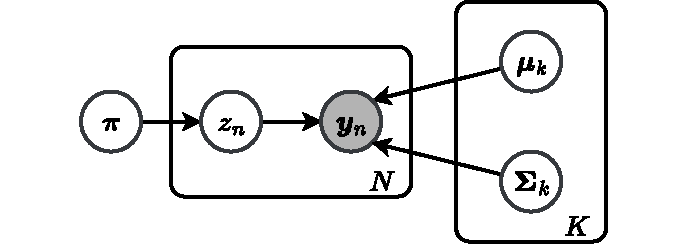
\includegraphics[width=0.5\textwidth]{figs/mixgaussian.pdf}
    \caption{A Gaussian mixture model represented as a graphical model}
    \label{fig:maxgaussian}
\end{figure}

\begin{example}
    \textbf{GMM represented as a graphical model}\\
    Viewing all variables, including model's parameters and obverations, 
    follow a generative story like Figure (\ref{fig:maxgaussian})
    {\small\begin{gather}
        p(\bm{y}_{1:N},\bm{z}_{1:N},\bm{\theta})
        = p(\bm{pi})
        \left[ \prod_{k=1}^K p(\bm{\mu}_k)p(\bm{\Sigma}_k) \right]
        \left[ \prod_{n=1}^N p(z_n|\bm{\pi})p(\bm{y}_n|z_n,\bm{\mu}_{1:K},\bm{\Sigma}_{1:K}) \right]
    \end{gather}}
    where latent variable $z_n\sim\text{Cat}(\bm{\pi})$ and model's parameters
    $\bm{\theta}=(\bm{\pi},\bm{\mu}_{1:K},\bm{\Sigma}_{1:K})$ are all unknown.
\end{example}


